\section{Stages of Development}\label{stages-of-development}

For a complete project there are fundamental stages that need to be
addressed, failure to address these stages can result in project drift
resulting in the end result not fulfilling expectations or failing to
achieve the requirements of the project.

It must be mentioned that although the term stages has been used, in
many methodologies especially those that involve rapid development many
of these stages will occur in either parallel or in quick succession;
for example testing will often happen throughout development to ensure
aspects of the code and design work as expected before extending the
software further.

\subsection{Analysis}\label{analysis}

The first stage of development is analysis, failing to analyse the
problem or obtain customer requirements renders development practically
impossible as the project scope can not be defined. Analysis often
requires the assessment of the problem or product to be developed and
rendering it down into more fundamental pieces such as how to implement
a RESTful API or store any data required. During this stage it is common
to perform competitor analysis by finding similar existing solutions to
challenges that may be faced and to implement improvements over the
competition and produce something objectively better to improve
usability, experience, performance and any combination of aspects that
can be deemed desirable.

\subsubsection{Competitors}\label{competitors}

\paragraph{\texorpdfstring{\href{http://sleep.urbandroid.org/}{Sleep as
Android}}{Sleep as Android}}\label{sleep-as-android}

This is the most feature packed alarm app available on Android that I
could find.

\subparagraph{Appearance}\label{appearance}

\begin{figure}
  \begin{center}
    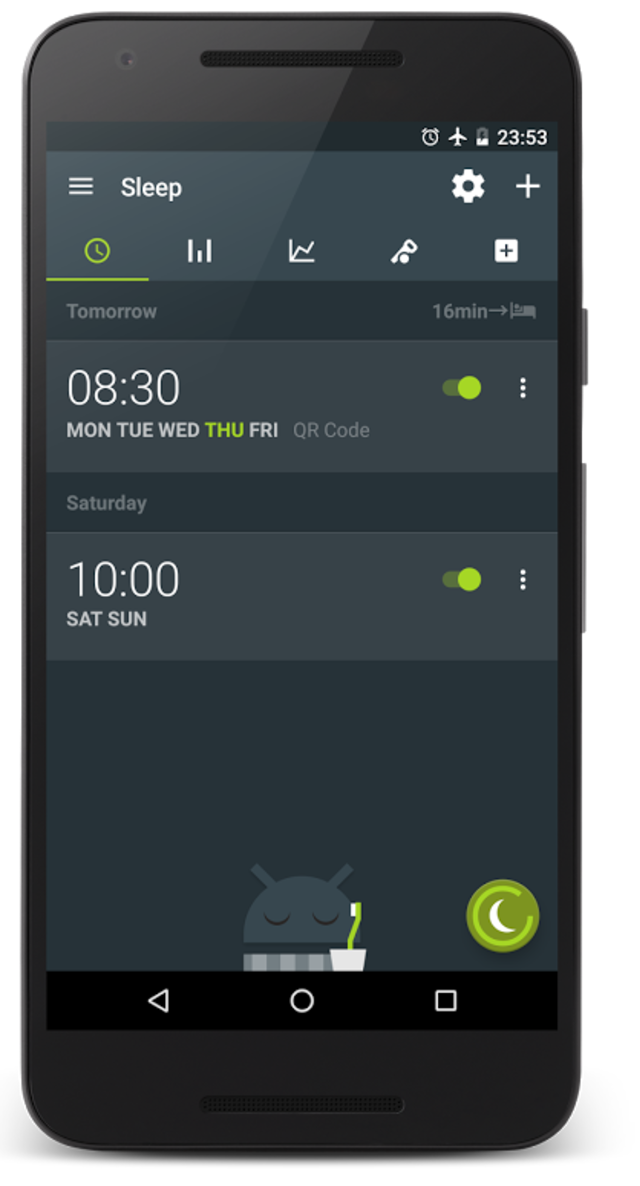
\includegraphics[scale=0.5,keepaspectratio]{Images/sleepas.png}
    \caption{Sleep as Android Screenshot}
  \end{center}
\end{figure}

The design of the app mostly follows the material guidelines set by the
Android development team with small variances in style. Overall the app
looks nice however some views can become crowded with information and
the number of features does make navigating the app harder than it needs
to be.

\subparagraph{Features}\label{features}

This app contains numerous features from the basics such as recurring
alarms to features such as solving a puzzle or scanning a QR code to
turn the alarm off. Features such as snore detection, sleep sensors and
sonar detection all detect and measure a persons sleep cycle and provide
statistics and graphs to assess the nights sleep and help inform the
user as how to improve their sleep quality, suggesting an earlier bed
time or to avoid sleeping aids and alcohol to prevent snoring.

\paragraph{\texorpdfstring{\href{https://cuckuu.com/}{Cuckuu}}{Cuckuu}}\label{cuckuu}

Cuckuu doesn't have the same level of integration with reminders,
appointments or weather as what I intend and it doesn't include any
smart bulb integration.

\subparagraph{Appearance}\label{appearance-1}

\begin{figure}
  \begin{center}
    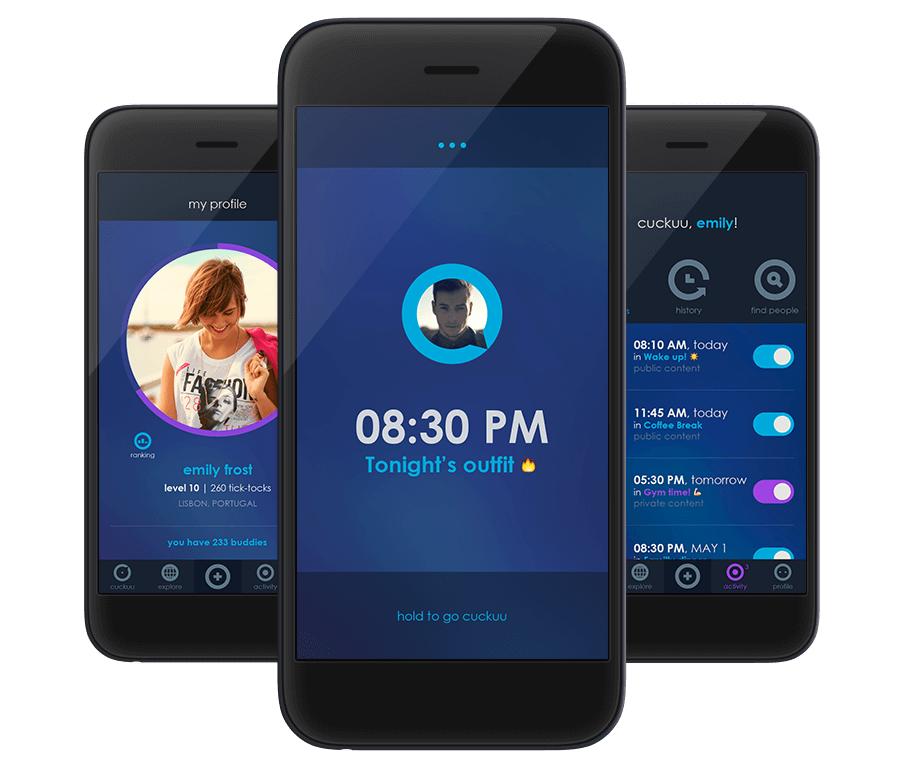
\includegraphics[scale=0.25,keepaspectratio]{Images/cuckuu.png}
    \caption{Cuckuu App Screenshots}
  \end{center}
\end{figure}

Cuckuu strikes a balance between Android and iOS allowing for it to be
available on both platforms, this is a good choice as it allows a user
to move between platforms and remain familiar with the design while
maintaining a good level of OS cohesion to keep the experience
consistent enough.

\subparagraph{Features}\label{features-1}

For Cuckuu social aspects of an alarm are the most important thing as
this is the apps unique selling point. Users are able to share alarms
(cuckuus) with their friends, possibly to alert them of shared events.

Users can add media or links to alarms both their own and shared alarms,
this provides a more visual and engaging alarm over a simple snooze and
off button. Another key aspect is a level of gamification towards alarms
by obtaining points for shutting of alarms quickly and providing a
leader-board among friends to encourage waking quickly and avoiding the
snooze button.

\paragraph{\texorpdfstring{\href{https://wakie.com/}{Wakie}}{Wakie}}\label{wakie}

Wakie is very different in how it intends to wake a user up and besides
being an alarm has little to what my app will consist of. Wakie does
have a very interesting concept though, that a stranger from around the
world will be able to call you when you would like to be woken and talk
about a topic you would like to discuss.

\paragraph{Appearance}\label{appearance-2}

\begin{figure}
\centering
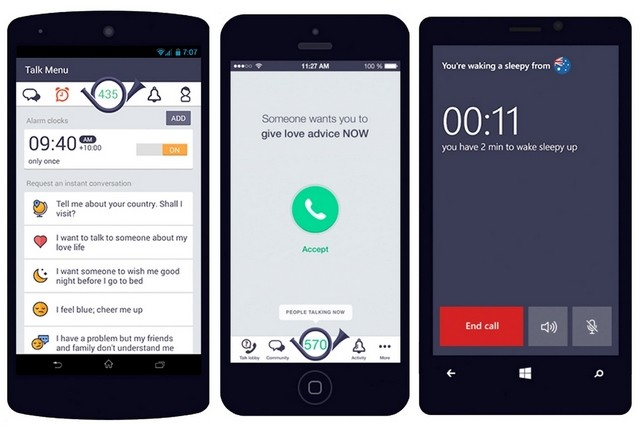
\includegraphics{Images/wakie.jpg}
\caption{Wakie App}
\end{figure}

With a very simple and clean design this app definitely looks nice and
allows itself to easily be ported into the varying mobile platforms.

\paragraph{Features}\label{features-2}

Since the initial analysis of this application the alarm aspects have
since been removed, as such I will be writing about the app in regards
to older versions that still contained the alarm functionality.

Overall the app works simply, you can set an alarm and another user of
the app will be connected to you through a phone call at the time the
alarm is set for. The concept is to provide a more sociable and personal
alarm, knowing that your alarm is a person on the other end possibly
encourages the user to wake up more than a simple alarm. The app and
it's functionality are free and only users of the app are connected
together.

\subsubsection{Problem Analysis}\label{problem-analysis}

Through my competitor analysis it is clear there is little competition
for smart-device connected alarm applications and with the increase in
smart-device popularity I feel there is a market for such an
application. The problems with existing alarm applications can be
attributed to their functionality, in some cases the amount of
functionality can be overwhelming in the case of \emph{Sleep as Android}
I feel there are just far to many features and this produces are
cluttered experience.

By focusing on a small amount of features such as how Wakie focuses on
an alarm with a chat, I intend to make a clean and simple app that is
familiar to the material design guidelines for the Android platform to
make my app blend seamlessly.

\subsection{Design}\label{design}

During the design stage the User Interface (UI) and various aspects of
the code are planned for development. By critically thinking about
certain design aspects with regards to the requirements outlined from
the analysis stage, designs of the software can be produced, this
includes both the visual designs of the user interface and some of the
software solutions that may be required such as certain tooling and
frameworks that are available for development to produce more stable
software faster by removing the need to produce custom solutions to
aspects that have been solved and are found throughout programming.

\subsubsection{Designs}\label{designs}

\emph{TODO} APPENDIX?

\subsection{Development}\label{development}

Throughout development everything that has been produced from both the
analysis and design stages are implemented through creation and
utilisation of software and assets such as images and sounds to produce
the goal of the project, in the instance of a mobile application this
would consist of producing and application that can run on the required
platforms such as Android, iOS or Windows Phone and for the application
to perform the tasks required such as sending and receiving messages and
displaying them to the user in the case of a communications application.

\subsubsection{Platform}\label{platform}

The development platform chosen is for Android devices, this is due to
the lead market share of mobile devices and through the relatively
simple and free development platform using Android studio and the
Android Virtual Device (AVD) tools provided, with the AVD providing the
ability to test applications on every version of Android available and
with different device specifications such as screen size, screen
density, on-board sensors and orientations.

With my personal phone being an Android device it is also possible to
install, test and debug my application on a physical device which is
often faster than a virtual device and can provide a better experience
of what the application will be when deployed.

\subsubsection{Target Market}\label{target-market}

Through various factors including my chosen platform, I will be
targeting the latest version of the Android platform 25 also known as
Nougat with support for devices as old as version 21 known as Lollipop.
My decision is based on the current version distribution statistics that
show over 50\% of devices are on versions 21 or higher and as such my
target is the majority share.

Version 19 (KitKat) currently hold a 20\% share which is a large
portion, however these are older devices that are likely to be from
poorer markets and due to the cost of smart-devices it is unlikely for
there to be a high demand of support from my app for KitKat. Due to the
release and support cycle provided by Google it is also likely for
KitKat to be unsupported by the end of the year and as such I feel there
are greater benefits to gain from the newer versions in place of using
older development features and supporting deprecated code.

Due to time limitations support will only be provided in English, with
the app having no alternative language support. From the restrictions
and targeted versions I will be focusing on countries that have English
as the native speaking language and areas of relative wealth as these
are the most likely to have access to the required smart-devices.

\subsection{Testing}\label{testing}

Often testing is an ongoing aspect of the development life cycle so that
as aspects of the application are developed tests and unit testing
classes are produced to allow the automation of testing. Performing
ongoing testing is useful to indicate that code is working correctly and
if during development if the automated testing indicates any issues
these can be resolved as they occur instead of during feedback or after
deployment, both of which increase development cost through having to
hunt down bugs and maintain the application during the life time of the
application.

\subsubsection{Tests}\label{tests}

The majority of testing involved will consist of introducing
functionality into the app and performing various actions to test that
functionality by using it as intended and trying to break it through
fringe cases and interactions that are likely to be less common such as
rapidly editing a text input or using input that is likely to be
uncommon such as number in place of text.

Further testing in the later stages of development will use others to
use the app and to provide feedback for their experience. It is very
difficult to test all cases as issues with UI or networking can be
intermittent and as such development should involve writing good code
and be less reliant on tests to indicate when something isn't working.

\subsection{Feedback}\label{feedback}

Feedback is crucial for assessing the success of a project, by obtaining
feedback from testers or trial users changes can be made to improve the
experience of the application. Feedback can be obtained during
development by having people use certain aspects of the application as
it's being developed. If during feedback multiple users raise complaints
about the same aspects this is a key indicator to change that aspect of
the application before full deployment to ensure a higher level of
polish and maintain a higher level of respect and image.

\subsubsection{User Trials}\label{user-trials}

As mentioned later stages of testing will involve others to test my app,
through testing I can obtain feedback for the design, usability and
highlight issues that I may not have accounted for in my development and
testing.
